\chapter{Hardware}
\label{Hardware}
Di seguito verranno descritte tutte le componenti hardware che sono servite al compimento della \textit{task}.\\
Il modulo GY-86, e il dispositivo di misura della distanza VL53L1X sono stati implementati sulla scheda STM32H745ZIQ, sulla quale, prima del \textit{merge} finale delle componenti fisiche, ogni componente è stata testata singolarmente.
\section{STM32 NUCLEO-H745ZI-Q}
L'STM32 NUCLEO-H745ZI-Q è una scheda di sviluppo prodotta da STMicroelectronics, basata sul microcontrollore STM32H745ZI-TQ6, 
appartenente alla famiglia ad alte prestazioni STM32H7. È progettata per facilitare lo sviluppo, il \textit{debug}, e la prototipazione di applicazioni 
\textit{embedded} complesse.\\
La NUCLEO-H745ZI-Q è stata utilizzata per sviluppo e \textit{testing} dei \textit{firmware} di gestione delle componenti di interesse.
Su di essa sono state caricate tutte le librerie software sviluppate con l'ausilio di STMCubeIDE.\\
\textbf{Caratteristiche principali:}
\begin{itemize}
    \item Architettura \textit{dual core}:
    \begin{itemize}
        \item processore ad alta prestazione \textit{Cortex}-M7, 480 [MHz].
        \item processore il cui utilizzo è consigliato per applicazioni \textit{real-time e low-power tasks, Cortex}-M4, 240 [MHz].
    \end{itemize}
        Questa architettura consente l'implementazione di applicazioni \textit{multithread} e la separazione funzionale tra il controllo ad alta frequenza e la gestione delle periferiche di comunicazione.\\
        Nel presente lavoro, l'esecuzione delle librerie software di gestione dei dispositivi di misura interessati è affidata al processore \textit{Cortex}-M4.
    \item Memoria
    \begin{itemize}
        \item 2 [Mb] di memoria \textit{Flash}.
        \item 1 [Mb] di memoria RAM, di cui 864 [KB] TCM SRAM (approfondimento disponibile nell'appendice A).
    \end{itemize}
    \item FPU, DSP, unità di protezione della memoria (MPU).  
%HMC5983
    \item Acceleratore grafico Chrom-ART (DMA2D).
    \item Possibilità di gestire \textit{interrupt ed eccezioni} di ogni genere efficientemente grazie alla presenza di un'unità di gestione dedicata, il NVIC (Nested Vector Interrupt Controller).\\
\end{itemize}
\textbf{Caratteristiche della scheda NUCLEO:}
\begin{itemize}
    \item Connettore ST Zio e Arduino Uno R3 per compatibilità \textit{shield}.
    \item Interfacce multiple di comunicazione seriale : USART, UART, I2C e SPI.
    \item Possibilità di creare applicazioni e eseguire attività direttamente legate allo scorrere del tempo reale tramite l'uso di una serie di \textit{timer} integrati. Questi ultimi, forniscono anche altre  \textit{features}, tra cui: \textit{input capture mode}, \textit{output compare mode}, generazione di impulsi singoli con larghezza e \textit{delay} programmabili, generazione di segnali ad impulso con modulazione della larghezza (PWM), generazione di accessi periodici alla memoria dinamica (DMA), contatore di eventi.
    \item \textit{Debugger} integrato ST-LINK/V3E via USB, con driver per il \textit{debug}, caricamento del \textit{firmware} nel microcontrollore e possibilità di comunicazione \textit{virtual COM}.
    \item Connettore USB Micro-B per programmazione e \textit{debug}.
    \item Alimentazione flessibile :
    \begin{itemize}
        \item Alimentazione via USB.
        \item Alimentazione tramite pin \textit{Vin}.
        \item Connettori esterni.
    \end{itemize}
    \item Capacità di eseguire sistemi operativi \textit{real-time} separatamente sui due core.
\end{itemize}
Nella seguente attività di sviluppo, al fine di comunicare con i dispositivi di misura, sono state utilizzate le periferiche di comunicazione seriale basate sul protocollo 
I2C fornite dal STM32H745ZIQ. \\
La verifica delle informazioni estrapolate dai sensori è avvenuta, come nel precedente caso, con comunicazione seriale, diverso è stato, però, il
protocollo di comunicazione utilizzato, UART. La periferica di comunicazione UART è stata gestita per poter visualizzare, tramite stampa video, controllata da un software di 
terze parti di nome \textit{Putty}, le informazioni estrapolate dai sensori.\\  
Al fine di manipolare le informazioni ottenute dai dispositivi di misura, è stato necessario utilizzare il \textit{timer} di sistema SysTick, System-Tick-Timer. Il timer
in questione viene configurato automaticamente dal CMSIS+HAL. Il suo utilizzo è ristretto alle funzioni HAL, che però, offrono al programmatore, una scorciatoia per lo sviluppo di applicazioni che hanno a che fare con il tempo reale.\\
L'alimentazione dei sensori è stata, anche'essa, affidata alla STM32H745ZIQ. La scheda, mediante i connettori presenti su di essa, riesce ad alimentare dispositivi la cui tensione di funzionamento rientra nei 5[V]. Presenta, di fatti, due uscite di alimentazione, una da 3.3[V] e una da 5[V]. L'unica utilizzata ai fini del progetto è stata l'uscita di alimentazione a 3.3[V]. Tutti i dispositivi supportano tale intervallo operativo.\\
Dopo lo sviluppo e la fase di testing, è stata raggiunto il livello di tolleranza di funzionamento desiderata dai dispositivi di misura. Con il concludersi del progetto, sono stati montati sul "Double Propeller Ducted-Fan" per gestire il funzionamento dei servomotori e motori.
 
\begin{figure}[H]
    \centering
    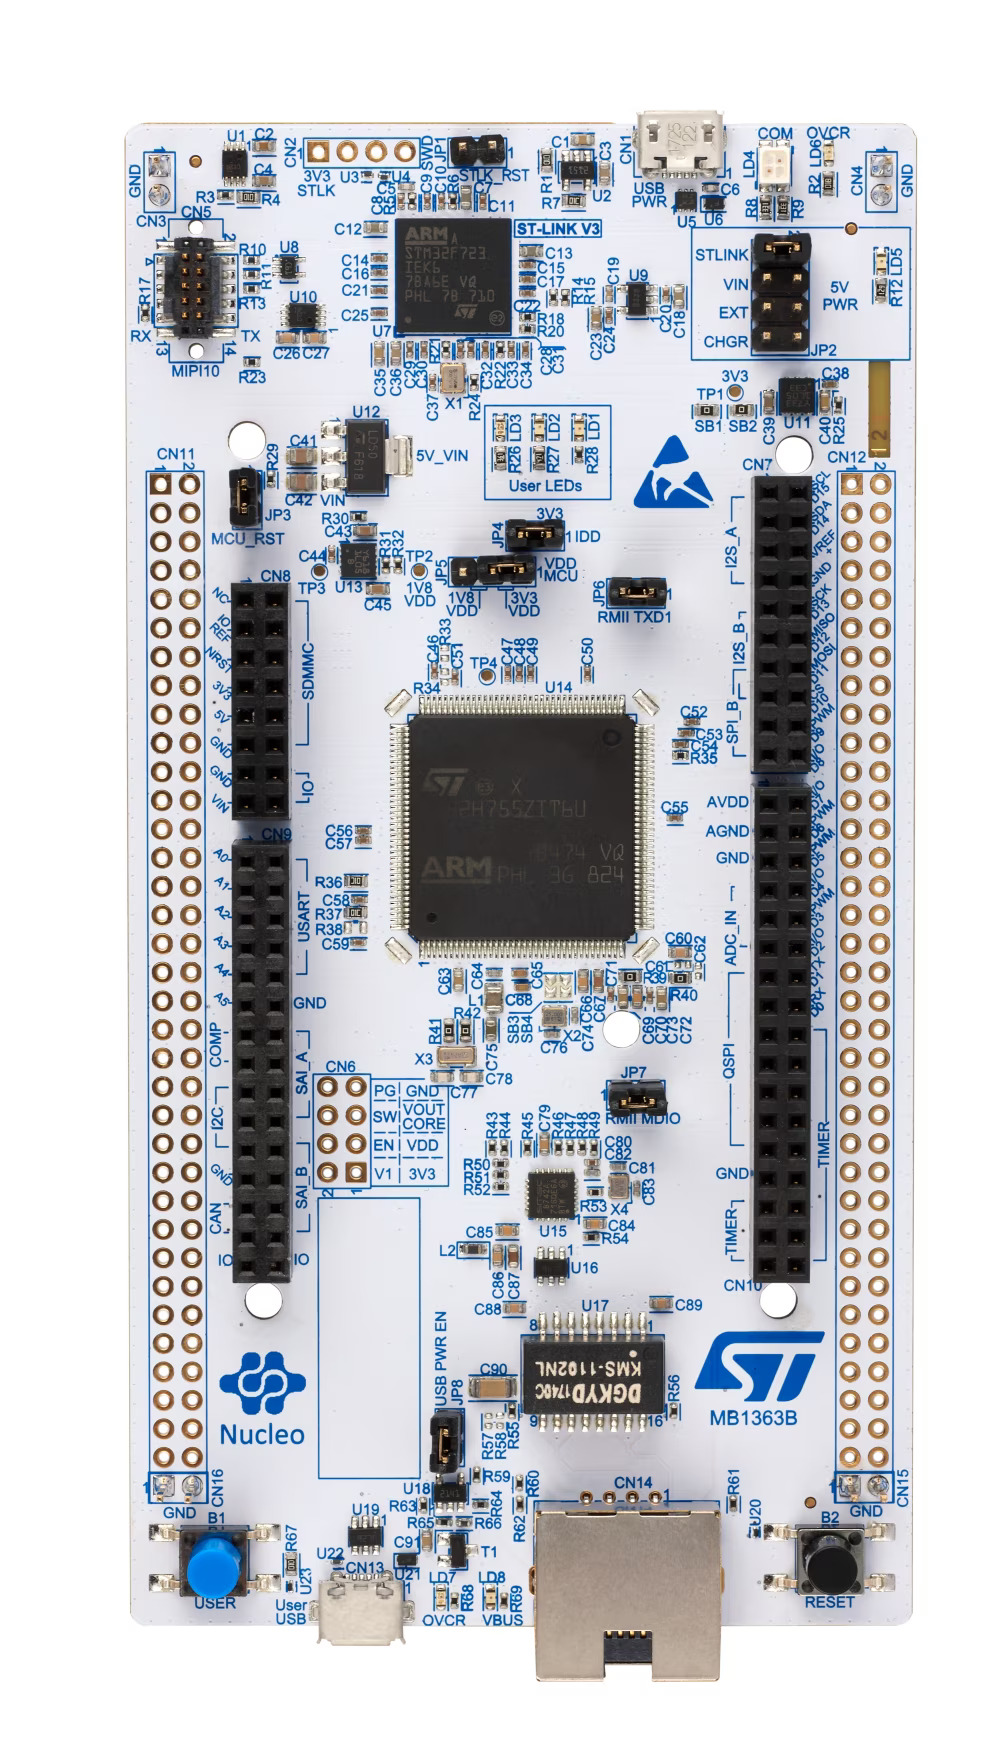
\includegraphics[width = 0.6\textwidth]{images/Immagine_1_relazione__IMMAGINE_STM32H745ZIQ.jpg}
    \caption{NUCLEO STM32-H745ZI-Q}
    \label{fig:etichetta}
\end{figure}
Per un controllo efficiente del Double Propeller Ducted-Fan, è necessaria la conoscenza della cinematica del sistema istante per istante.
L'effettiva conoscenza della cinematica, passa attraverso l'estrapolazione di informazioni da dispositivi capaci di percepire: accelerazione, velocità, posizione e orientamento del sistema interessato.
Per realizzare quest'ultimo interesse, si è optato per l'unità di misura inerziale GY-86, e il sensore di misura della distanza VL53L1X.\\
Nei paragrafi a venire, verranno descritte le caratteristiche dei dispositivi, utilizzate per adempiere all'obiettivo primario.
%fino a qui corretttti gli errori  HMC5983
\section{Modulo GY-86. Unità di misura inerziale}
Al fine di ottenere una struttura compatta, è necessaria la ricerca di un circuito integrato che contiene, sia un accelerometro che un giroscopio, e anche un magnetometro. Per rispettare tale descrizione, si è optato per il modulo GY-86, contenente l'MPU6050 InvenSense e l'HMC5983 Honeywell.
In seguito, un listato delle caratteristiche di funzionamento sfruttate ai fini del progetto.\\\\
\textbf{Caratteristiche principali:}
\begin{itemize}
\item Alimentazione da 3-5 [V].
\item dimensioni : 22 x 17 [mm].
\item Protocollo di comunicazione standard I2C. Supporta una comunicazione I2C fino a\\400 [kHz], "Fast-mode".
\item Un LED di colore verde è utilizzato per segnalare l'avvenuta alimentazione del sistema.
\end{itemize}
Le caratteristiche elencate nel listato precedente, sono comuni a tutti i dispositivi appartenenti al modulo. Pertanto non verranno ripetute nelle descrizioni a seguire. 
    \section{MPU6050 InvenSense}
    L'MPU6050 InvenSense è il primo dispositivo di misura inerziale al mondo a sei assi. Combina un accelerometro a tre assi e un giroscopio a tre assi.\\
    In seguito un elenco delle caratteristiche dell'oggetto che sono state sfruttate nel progetto.\\
    \textbf{Caratteristiche:}
    \begin{itemize}
    \item Alimentazione da 2.375-3.46 [V]. L'alimentazione è gestita dal modulo.
    \item Dimensioni : 4 x 4 x 0.9 [mm].
    \item Possiede un \textit{bus} I2C interamente dedicato all'accettare \textit{input} da una bussola esterna a  tre assi.  
    \item Possiede tre convertitori analogici-digitali per componente (ADCs). La risoluzione di questi è a 16 [bit]. Ottenendo così la digitalizzazione del segnale di uscita del giroscopio e accelerometro.
    \item Tolleranza agli \textit{shock} fino a 10.000 [g]. % convertitore analogico-digital a 16 bit
    \item \textit{Digital Low-Pass Filter} programmabile sia per l'accelerometro che per il giroscopio.
    \end{itemize}
Nel paragrafo seguente verranno descritte le caratteristiche specifiche dell'accelerometro e del giroscopio. Prima però, è opportuna una spiegazione di come questi sensori acquisiscono le misure.
\subsection{Il principio di misura dell'accelerometro e del giroscopio}
\subsubsection{Accelerometro}
L'accelerometro integrato nel dispositivo MPU6050 InvenSense è di tipo capacitivo MEMS, \textit{Micro-Electro-Mechanical Systems}, e consente la misura dell'accelerazione lungo i tre assi cartesiani.\\
Il principio di funzionamento si basa sulla rilevazione delle variazioni di capacità tra microstrutture mobili e fisse realizzate su un substrato di silicio.\\
L'elemento sensibile di ciascun asse è costituito da una massa sospesa, \textit{proof mass}, vincolata da microtravi elastiche ad una cornice ancorata al substrato.
In condizioni di quiete, la massa è in equilibrio e la capacità tra le \textbf{piastre interdigitate*} rimangono simmetriche.\\
Quando il dispositivo è sottoposto ad un'accelerazione lungo uno degli assi sensibili, la massa inerziale si sposta in direzione opposta a quella dell'accelerazione, generando una variazione differenziale 
della capacità tra le piastre.\\
La variazione di capacità viene rilevata da un circuito integrato, che la converte in un segnale elettrico, proporzionale alla velocità applicata.\\
Il segnale analogico prodotto, viene successivamente digitalizzato da un convertitore analogico-digitale a 16 bit, integrato nel chip.
%riprendi controllo da qui 
\subsubsection{Giroscopio}
Il giroscopio integrato nel dispositivo MPU6050 InvenSense è un sensore MEMS di tipo vibrante, \textit{vibrating structure gyroscope}, e consente la misura della velocità angolare lungo i tre assi cartesiani.\\
Il principio di funzionamento si basa sull'effetto Coriolis, che si manifesta quando una massa in moto oscillatorio subisce una rotazione rispetto ad un sistema di riferimento inerziale.\\
All'interno del sensore, ciascun asse dispone di una o più masse vibranti, le quali vengono mantenute in oscillazione a frequenza costante, mediate un circuito di attuazione elettrostatica. Quando il dispositivo ruota attorno ad uno 
degli assi, la massa subisce una forza di Coriolis data da:

\begin{equation}
    \vec{F_c} = 2m(\vec{v}\,\times \,\vec\omega )
\end{equation}
dove \textit{m} è la massa oscillante, $\vec{v}$ è la velocità della massa nella sua traiettoria vibrante, $\vec{w}$ è la velocità angolare del corpo.\\
Questa forza induce uno spostamento trasversale rispetto alla direzione di vibrazione, che viene rilevato attraverso variazioni di capacità tra elettrodi fissi e mobili, similmente a quanto avviene nell'accelerometro.\\
Tali variazioni, proporzionali alla velocità angolare, vengono convertite in un segnale elettrico mediante un circuito di lettura differenziale e successivamente digitalizzate tramite ADC integrato.
\subsection{Accelerometro a tre assi}
L'MPU6050 InvenSense include un accelerometro a tre assi.\\
Il dispositivo utilizza la tecnologia MEMS.\\
Generalmente, l'accelerometro è un dispositivo che fornisce misure sull'accelerazione percepita lungo i tre assi cartesiani.\\
Nel nostro caso, dopo una corretta manipolazione delle informazioni estrapolate, il dato ottenuto rappresenta l'accelerazione in [g], sui tre assi cartesiani.\\
In seguito, un listato descrivente le specifiche caratteristiche, sfruttate ai fini del progetto.\\\\\\\\
\textbf{Caratteristiche specifiche:}
\begin{itemize}
\item L'accelerometro a tre assi fornisce un \textit{output} digitale con \textit{"Full Scale Range"} programmabile dall'utente.\\ Abbiamo quattro diversi \textit{"Full Scale Range"}. Questi sono i \textit{range} dinamici della misura, indicano il massimo valore di accelerazione che può essere misurato lungo i tre assi. Alla fine del paragrafo è stata inserita una tabella che descrive i vari \textit{"Full Scale Range"} dell'accelerometro. 
\item Valore normale di corrente per l'operatività : $500\,[\mu\text{A}]$. Caratteristica gestita dal modulo GY-86.
\item Frequenza di acquisizione delle misure : 1 [kHz].
\item Rilevamento e segnalazione dell'orientamento.
\item Possibilità di effettuare \textit{Self-Test}.
\end{itemize}

\begin{table}[H]
    \centering
    \resizebox{\textwidth}{!}{
    \begin{tabular}{|c|c|c|c|c|}
        \hline 
        \textit{Full Scale Range} & Utilizzo consigliato & Sensibilità & Vantaggi & Svantaggi \\
        \hline
        $\pm 2[g]$ & Applicazioni di alta precisione & Alta : 16384 [LSB]/g & Alta precisione & Rapida saturazione\\
        \hline
        $\pm 4[g]$ & Movimenti Moderati & Media : 8192 [LSB]/g & Buon compromesso & /\\
        \hline
        $\pm 8[g]$ & Attività dinamiche. (Corsa, Robotica mobile) & Bassa : 4096 [LSB]/g & Ampio range & minore precisione\\
        \hline
        $\pm 16[g]$ & Urti, vibrazioni intense, cadute & Molto bassa : 2048 [LSB]/g & Bassa saturazione & precisione scarsa\\
        \hline
    \end{tabular}
    }
    \caption{Full Scale Range Accelerometro}
    \label{tab: tabella}
\end{table}
% peridita
\subsection{Giroscopio a tre assi}
MPU6050 InvenSense include anche un giroscopio a tre assi. Il giroscopio, anch'esso costruito sul disegno della tecnologia MEMS, fornisce misure sulla velocità angolare lungo i tre assi cartesiani.\\
Nel nostro caso, la velocità angolare è espressa in [°/s] (gradi al secondo).\\
A seguire, un elenco descrivente le caratteristiche specifiche, sfruttate ai fini del progetto.\\\\
\textbf{Caratteristiche specifiche:}
\begin{itemize}
\item Il giroscopio a tre assi fornisce un output digitale con \textit{"Full Scale Range"} programmabile dall'utente.\\Anche in questo caso abbiamo quattro diversi \textit{"Full Scale Range"}. Questi, sono i \textit{range} dinamici della misura, indicano il massimo valore di velocità angolare che può essere misurato sui tre assi cartesiani.\\Alla fine del paragrafo, è stata inserita una tabella che descrive i vari \textit{"Full Scale Range"} del giroscopio.
\item Valore normale di corrente per l'operatività : 3.6 [mA].
\item Valore normale di corrente in \textit{standby} : $5\,[\mu\text{A}]$
\item Il sensore fornisce una migliorata stabilità del \textit{bias} e della sensibilità rispetto alla temperatura, che si traduce in una ridotta necessità di calibrazione da parte dell'utente.
\item Buone prestazioni in termini di rumore alle basse frequenze.
\item \textit{"Digital Low-Pass Filter"} programmabile.
\item Frequenza di acquisizione delle misure : 8 [kHz].
\item Possibilità di frazionare la frequenza standard di acquisizione delle misure.
\item Possibilità di effettuare \textit{Self-Test}.
\end{itemize}

\begin{table}[H]
    \centering
    \resizebox{\textwidth}{!}{
    \begin{tabular}{|c|c|c|c|c|}
        \hline 
        \textit{Full Scale Range} & Utilizzo consigliato & Sensibilità & Vantaggi & Svantaggi \\
        \hline
        $\pm 250[°/s]$ & Movimenti lenti e precisi & Alta : 131[LSB]/[°/s] & Alta precisione & Rapida saturazione\\
        \hline
        $\pm 500[°/s]$ & Movimenti moderati(droni a bassa velocità) & Media : 65.5 [LSB]/[°/s] & Buon compromesso & /\\
        \hline
        $\pm 1000[°/s]$ & Movimenti rapidi  & Bassa : 32.8 [LSB]/[°/s] & Ampio range & perdita di dettaglio\\
        \hline
        $\pm 2000[°/s]$ & Rotazioni veloci, urti angolari & Molto bassa : 16.84 [LSB]/[gradi/s] & Bassa saturazione & precisione scarsa\\
        \hline
    \end{tabular}
    }
    \caption{Full Scale Range Giroscopio}
    \label{tab: tabella}
\end{table}
L'obiettivo finale dei test è quello di verificare il corretto funzionamento del sensore e delle librerie sviluppate per gestirlo. La verifica è avvenuta per ogni \textit{Full Scale Range}.

\section{HMC5883L Honeywell}
Lavoro attribuito a Matteo Vitullo

\begin{figure}[H]
    \centering
    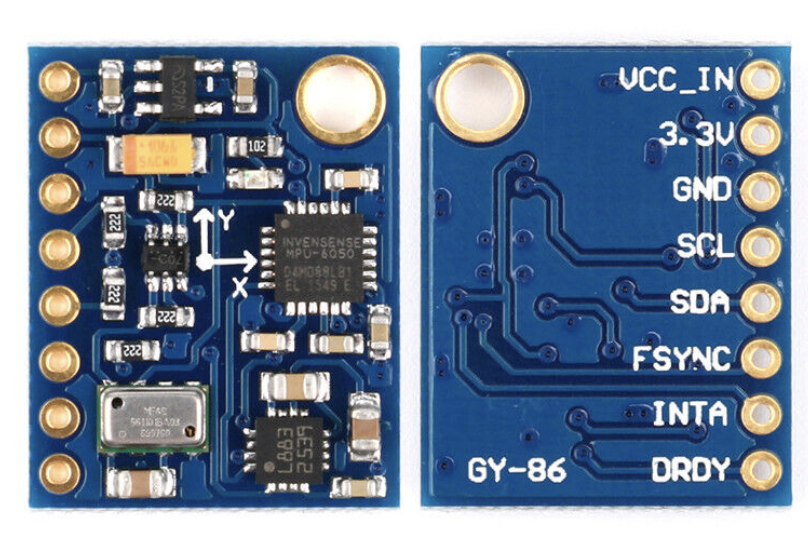
\includegraphics[width = 0.6\textwidth]{images/Immagine_2_modulo_GY_86.png}
    \caption{Modulo GY-86}
    \label{fig:etichetta}
\end{figure}

\section{VL53L1X ST. Sensore Time-of-Flight per la misurazione a lunga distanza}
Per il desiderato comportamento del \textit{Ducted-Fan}, è necessario conoscere la distanza da terra mentre quest'ultimo è in volo. Bisogna, dunque, includere un sensore apposito.\\
Il VL53L1X di STMicroelectronics è pienamente coerente con i requisiti precedentemente espressi.\\
Tuttavia, non si è optato per l'integrazione diretta del sensore della casa STMicroelectronics, si è preferito acquistare il modulo \textit{"iris11a 0J9776"} prodotto da \textit{Pololu}.
Il modulo \textit{breakout} di Pololu, contenente il sensore VL53L1X di STMicroelectronics, è stato scelto per semplificare la fase di configurazione elettronica del sensore.\\
Per comprendere il suo principio di misura, è opportuno dedicare un'intera sezione alla sua descrizione.

\subsection{Il principio di misura \textit{Time-of-Flight}, ToF}
Il principio di misura \textit{Time-of-Flight} si basa sulla determinazione del tempo impiegato da un segnale, generalmente un impulso luminoso nella banda dell'infrarosso, per compiere
un viaggio di andata e ritorno tra un emettitore e un bersaglio riflettente. In particolare, per il nostro dispositivo di misura VL53L1X, la sorgente di emissione luminosa è costituita da
un laser a cavità verticale (VCSEL), che emette brevi impulsi di luce modulata.
Il segnale emesso si propaga nell'ambiente fino ad incontrare un oggetto. Parte della radiazione viene riflessa e raccolta da un rilevatore sensibile alla luce, in genere un array SPAD,
\textit{"Single-Photon Avalanche Diode"}. Questo rilevatore è in grado di registrare l'arrivo anche di singoli fotoni, consentendo una misura estremamente sensibile del tempo di volo.\\
Una volta noto l'intervallo temporale tra l'istante di emissione dell'impulso e quello di ricezione del suo \textit{"eco"}, il calcolo della distanza si ottiene applicando la relazione:
\begin{equation}
    d = \frac{c \cdot \Delta t}{2}
\end{equation}
dove \textit{d} è la distanza dell'oggetto dalla superficie, \textit{c} è la velocità della luce nel vuoto e $\Delta t$ è il tempo di volo misurato. Il fattore 2 al denominatore tiene conto
che il segnale percorre il tragitto due volte, andata e ritorno.\\
I ToF moderni possono utilizzare tecniche avanzate di correlazione temporale o modulazione di fase per migliorare la precisione e la resistenza al rumore ambientale.\\
Nel caso in esame,  il VL53L1X di ST utilizza la tecnologia base ToF o dTof, \textit{"Direct Time-of-Flight"}.\\
\subsection{VL53L1X STMicroelectronics. Caratteristiche}
In seguito, un listato delle principali caratteristiche tecniche del VL53L1X di ST, sfruttante per il progetto.\\
\paragraph{Caratteristiche}
\begin{itemize}
\item Dimensioni : 4.9 x 1.25 x 1.56 [mm]
\item Valore della tensione di alimentazione : 2.6-3.5 [V].
\item Escursione di temperatura per la corretta operatività : da -20 a 85 [°C].
\item Emettitore ad infrarossi di classe [1], di lunghezza d'onda : 940 [nm]. \\Un Laser di classe [1] è un emettitore di onde elettromagnetiche, le cui condizioni operative normali, sono considerate sicure per l'occhio umano e la pelle.
\item Misurazione accurata e veloce. Il dispositivo riesce a misurare distanze fino ai 4 [m] ad una frequenza di acquisizione di 50 [Hz].
\item \textit{Full Field-of-view} standard di 27 [°].
\item \textit{Region-of-interest} (ROI) programmabile. Questa \textit{feature} permette di ridurre il FoV.
\item Presenza di pin di \textit{ShutDown} e di \textit{interrupt}.
\item Sfrutta il protocollo di comunicazione seriale I2C fino a 400[kHz], \textit{Fast-Mode}.
\end{itemize}
Il VL53L1X, come MPU6050, possiede diversi intervalli a piena scala da sfruttare a seconda delle necessità.
\begin{table}[H]
    \centering
    \resizebox{\textwidth}{!}{
    \begin{tabular}{|c|c|c|}
        \hline 
        \textit{Modalità} & Range massimo in codizioni di scarsa luce (approssimato) & Range massimo con luce ambientale \\
        \hline
        \textit{Short} & 136 [cm] & 135 [cm]\\
        \hline
        \textit{Medium} & 290 [cm] & 76 [cm]\\
        \hline
        \textit{Long} & 360 [cm] & 73 [cm]\\
        \hline
    \end{tabular}
    }
    \caption{\textit{Distance mode} del VL53L1X STMicroelectronics.}
    \label{tab: tabella}
\end{table}
\begin{center}
    \footnotesize \textit{Tabella ricavata sotto le seguenti condizioni : \textit{timing budget} = 100 [ms], bersagio bianco, riflettanza : 88\%, luce ambientale : 200 [kcps/SPAD].}
\end{center}

\begin{figure}[H]
    \centering
    \begin{minipage}{0.45\textwidth}
        \centering
        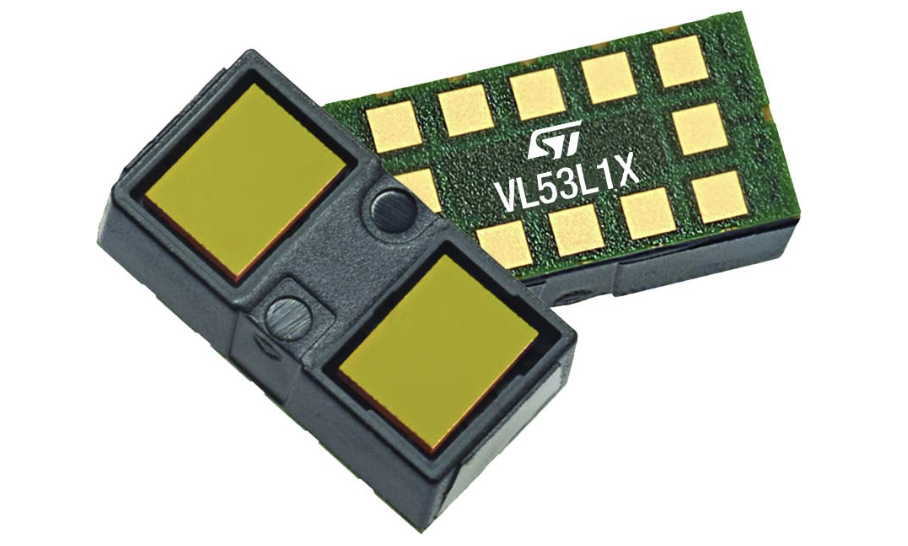
\includegraphics[width=\textwidth]{images/Immagine_3_VL53L1X.png}
        \caption{VL53L1X STMicroelectronics}
        \label{fig:img1}
    \end{minipage}
    \hfill
    \begin{minipage}{0.45\textwidth}
        \centering
        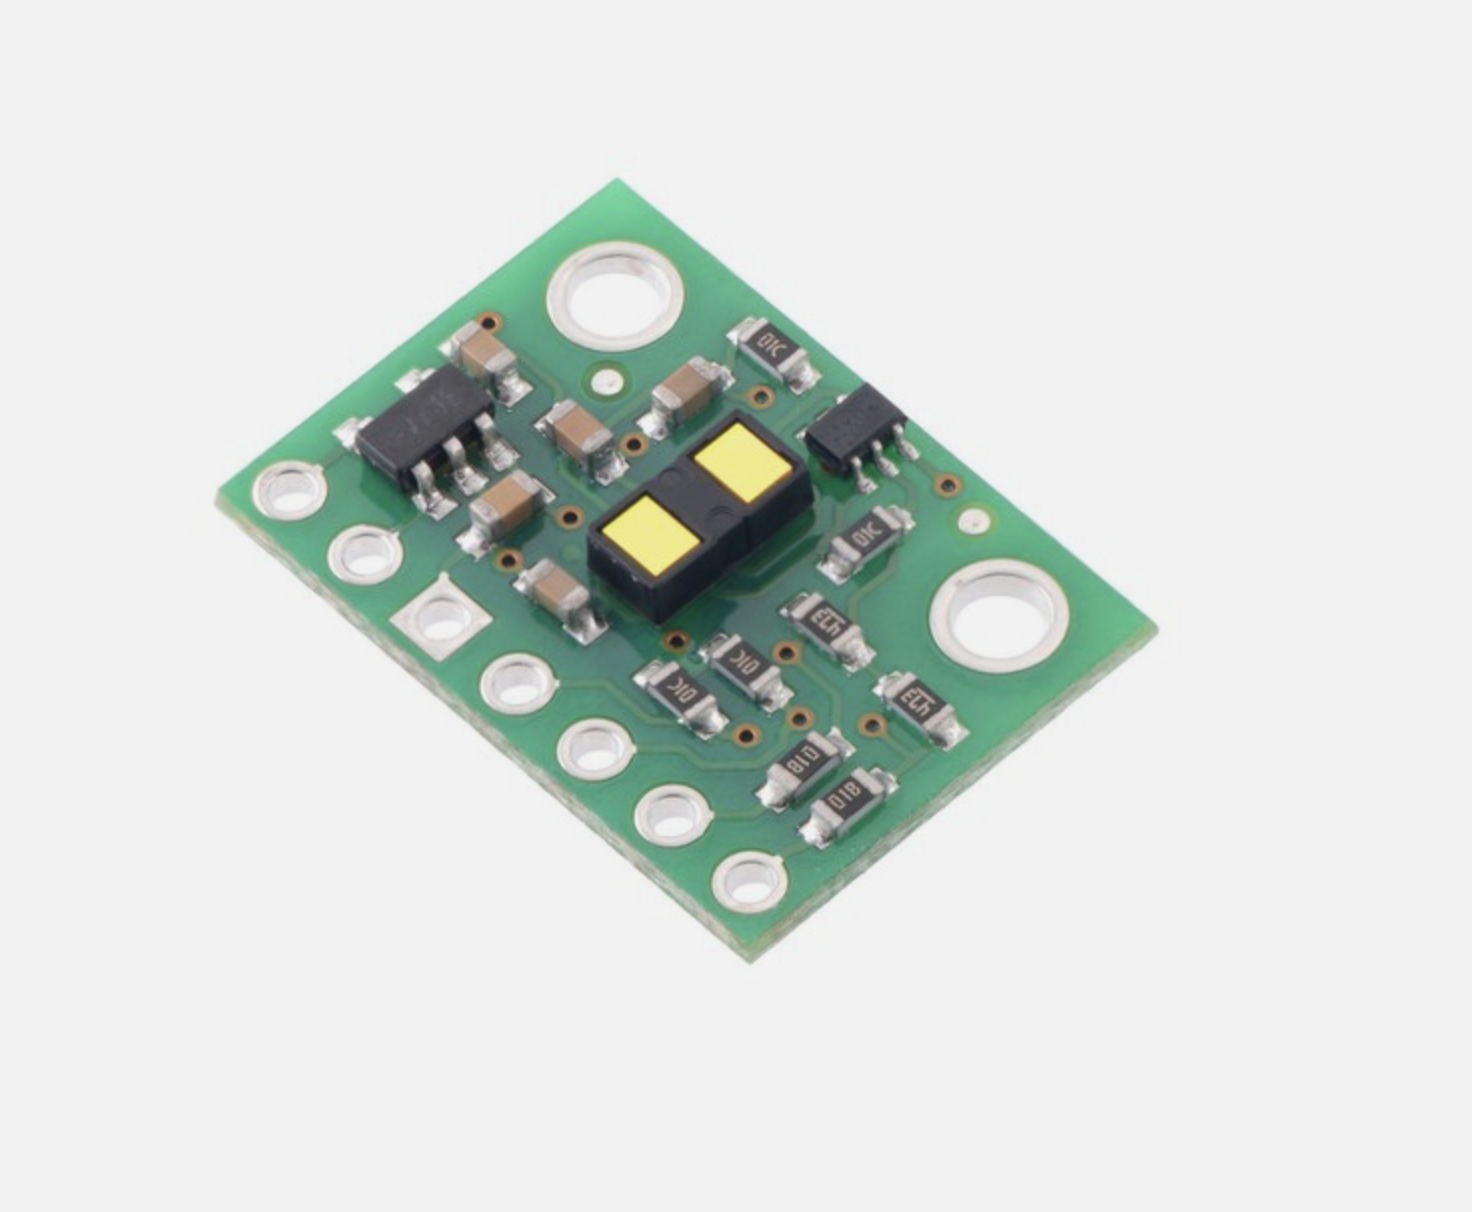
\includegraphics[width=\textwidth]{images/Immagine_4_Pololu.png}
        \caption{Modulo iris11a 0J9776 Pololu contenente il VL53L1X STMicroelectronics}
        \label{fig:img2}
    \end{minipage}
\end{figure}
%qui
\section{Schema dei collegamenti}
Nel sottostante schema è possibile visualizzare lo schema dei collegamenti.
\subsubsection{Modulo GY-86}
Per il GY-86 è stata utilizzata la periferica di comunicazione "I2C1" offerta dalla NUCLEO-H745ZI-Q.
\begin{itemize}
\item VCC del GY-86 collegato al CN8 pin 7   della NUCLEO-H745ZI-Q (3.3[V]).
\item GND del GY-86 collegato al CN8 pin 11  della NUCLEO-H745ZI-Q (GND).
\item SCL del GY-86 collegato al CN10 pin 14 della NUCLEO-H745ZI-Q (PB6).
\item SDA del GY-86 collegato al CN10 pin 16 della NUCLEO-H745ZI-Q. (PB7).
\end{itemize}
\subsubsection{Modulo iris11a 0J9776 Pololu}
Diversamente, per il modulo in questione, è stata utilizzata la periferica di comunicazione "I2C2" offerta dalla NUCELO-H745ZI-Q.
\begin{itemize}
\item VIN del Pololu collegato al CN7 pin 7   della NUCLEO-H745ZI-Q (PB12).
\item GND del Pololu collegato al CN8 pin 13  della NUCLEO-H745ZI-Q (GND).
\item SCL del Pololu collegato al CN10 pin 32 della NUCLEO-H745ZI-Q(PB10).
\item SDA del Pololu collegato al CN10 pin 34 della NUCLEO-H745ZI-Q.(PB11)
\item XSHOUT del Pololu collegato al CN9 pin 29 della NUCLEO-H745ZI-Q (PB14).
\end{itemize}

\begin{figure}[H]
    \centering
    \includegraphics[width=1\textwidth,keepaspectratio]{images/SchemaCollegamentiDrone.drawio.png}
    \caption{Schema dei collegamenti}
    \label{fig:schema}
    \end{figure}
